\documentclass[10pt]{article}

\usepackage[margin=0.75in]{geometry}
\usepackage{fancyhdr}
\pagestyle{fancy}
\usepackage{amsmath}
\usepackage{amssymb}
\usepackage{color}

\definecolor{mygreen}{rgb}{0,0.6,0}
\definecolor{mygray}{rgb}{0.5,0.5,0.5}
\definecolor{mymauve}{rgb}{0.58,0,0.82}

\usepackage{graphicx}
\usepackage{listings}
\lstset{language=Python,
		keywordstyle=\color{blue},
		commentstyle=\color{mygreen},
		numbers=left,
		numbersep=5pt,
	    numberstyle=\color{mymauve}, % the style that is used for the line-numbers
        rulecolor=\color{green},         
        showspaces=false,                
  		showstringspaces=false,          % underline spaces within strings only
  		showtabs=false,                  % show tabs within strings adding particular underscores
  		stepnumber=1}

\allowdisplaybreaks

\lhead{FEM 5168 HW1}
\chead{Melvyn Ian Drag}
\rhead{\today}
\setlength{\parskip}{0pt} 
\setlength{\parindent}{0pt}
\newcommand{\tab}[1]{\hspace*{4ex}\rlap{#1}}
\newcommand{\tbf}[1]{\textbf{#1}}
\newcommand{\ptl}[2]{\frac{d^2 #1}{d #2 ^2}}
\newcommand{\pl}[2]{\frac{d #1}{d #2}}
\newcommand{\iab}[2]{\int_#1^#2}
\begin{document}
\section*{Problem 1}
\tbf{A)}\begin{gather*}
u(0) = 0 - \frac{sinh(0)}{sinh(1)} = 0\\u(1) = 1 - \frac{sinh(1)}{sinh(1)} = 0\\
u'(x) = 1 - \frac{cosh(x)}{sinh(1)}\\
u''(x) = -\frac{sinh(x)}{sinh(1)}\\
\therefore -u''(x) + u = \frac{sinh(x)}{sinh(1)} + x - \frac{sinh(x)}{sinh(1)} = x
\end{gather*}
\tbf{B)}\begin{gather*}
\Bigg(-\ptl{u}{x}+u\Bigg)v=xv\textrm{ for }v\in \mathcal{H}_0^1\\
\iab{0}{1}-\ptl{u}{x}v+uv\;dx = \iab{0}{1}xv\;dx\\
\iab{0}{1}\pl{u}{x}\pl{v}{x}\;dx+\iab{0}{1}uv\;dx = \iab{0}{1}xv\;dx
\end{gather*}
\tbf{C)} The code for these next two sections is long. It is attached as an appendix.
\begin{center}
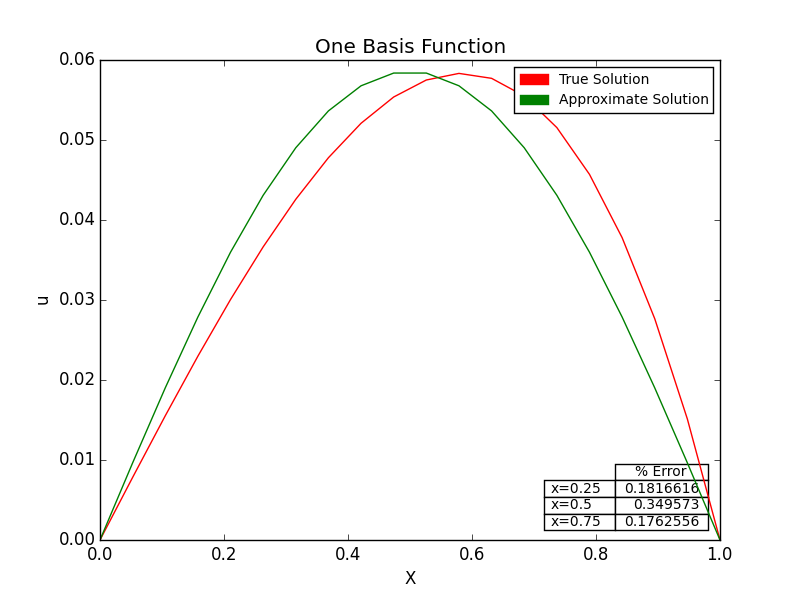
\includegraphics[scale=0.4]{one.png}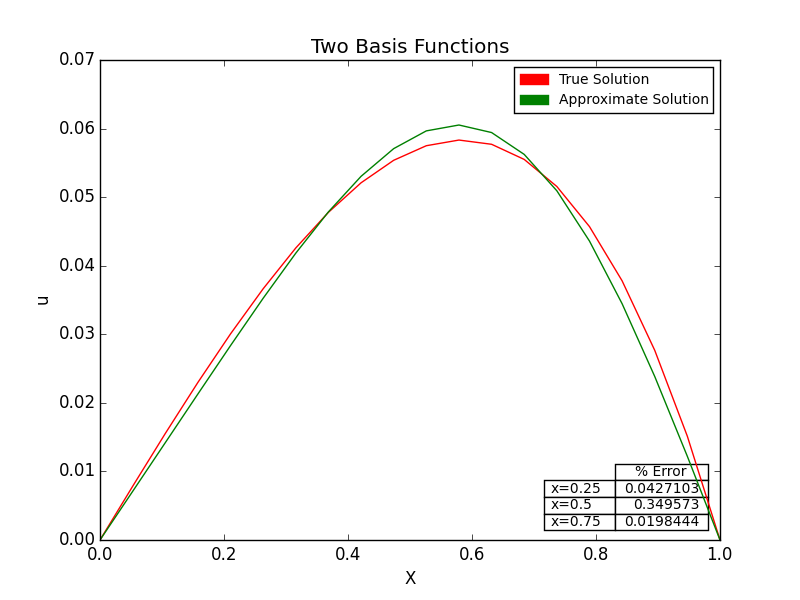
\includegraphics[scale=0.4]{two.png}
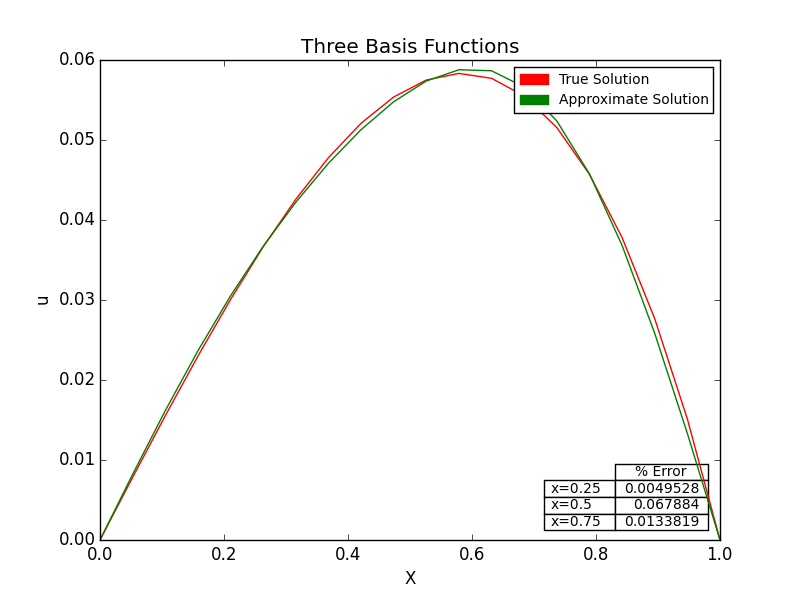
\includegraphics[scale=0.4]{three.png}
\end{center}
\newpage
\tbf{D)}
\begin{center}
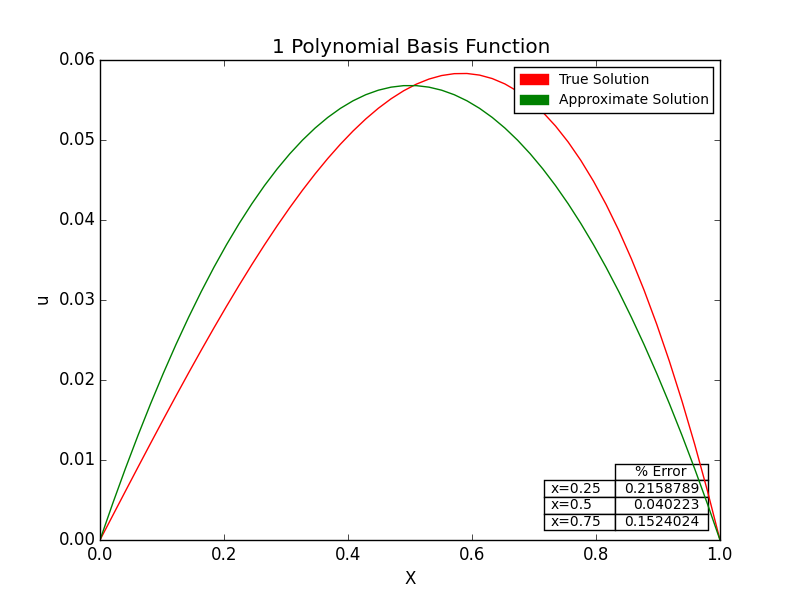
\includegraphics[scale=0.4]{one_poly.png}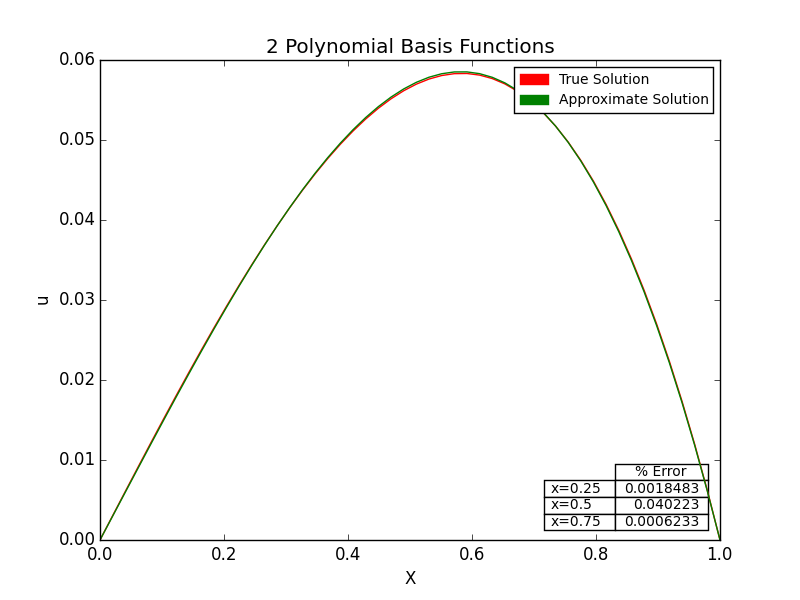
\includegraphics[scale=0.4]{two_poly.png}
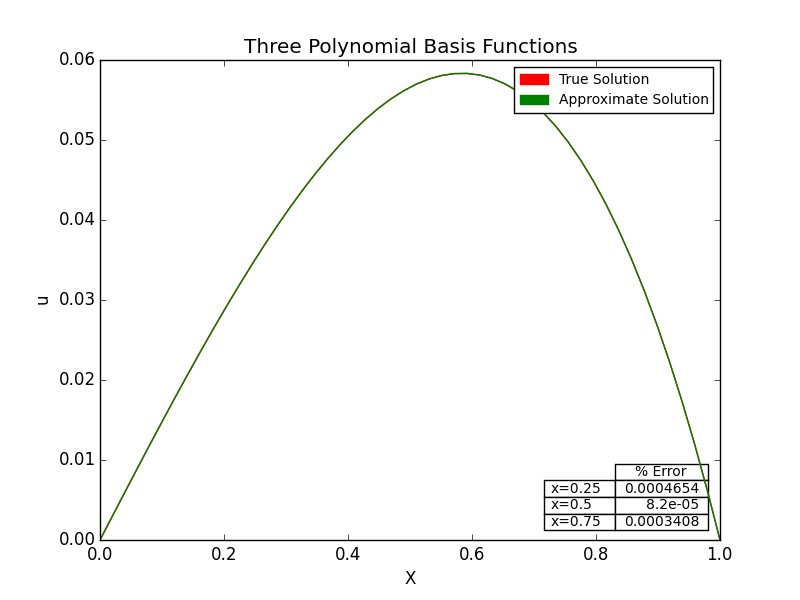
\includegraphics[scale=0.4]{three_poly.png}
\end{center}
\section*{Problem 2}
\tbf{A)} We are solving $\iab{0}{1}\pl{v_i}{x}\pl{u}{x}dx=\iab{0}{1}xv_i dx$ given a set of test functions $\{\sin(k\pi x)\}_{k=1}^n$. We have: 
\begin{equation*}
\frac{d}{dx}\sin(k\pi x)=k\pi \cos(k\pi x)
\end{equation*}
and then notice that the $ij^{th}$ entry in the stiffness matrix \textbf{K} is $\iab{0}{1}ij\pi^2\cos(i\pi x)\cos(j\pi x)dx$, $i, j\in \{1, 2, \dots, n\}$. The set $\{\cos(k\pi x)\}_{i=1}^n$ is an orthogonal set. Therefore, all of the nondiagonal entries are 0. 
The diagonal entries all integrate to $\frac{i^2\pi^2}2$. We integrate the $i^{th}$ element of the load vector, $\iab{0}{1}x\sin(i\pi x)dx = -\frac{\cos(i\pi)}{i\pi} = \frac{(-1)^{i+1}}{i\pi}$. Then we solve the system by dividing load vector elements by their corresponding diagonal elements and get $\alpha_i=\frac{2(-1)^{i+1}}{i^3\pi^3}$.

\tbf{B)} The exact solution is found by integrating twice and applying the boundary conditions. We find the exact solution is $u(x) = -\frac{x^3}{6}+\frac{x}{6}$. My code finds $\vec{\alpha} = (0.25, 0.1666) = (\frac14, \frac16)$. When we substitute these as the coefficients of $u_N$:
\begin{gather*}
\frac14(x(1-x)) + \frac16(x(1-x)(\frac12 - x))=-\frac{x^3}{6}+\frac{x}{6}
\end{gather*}
As it turns out, the Galerkin Method can yield the exact solution to a problem.
\begin{center}
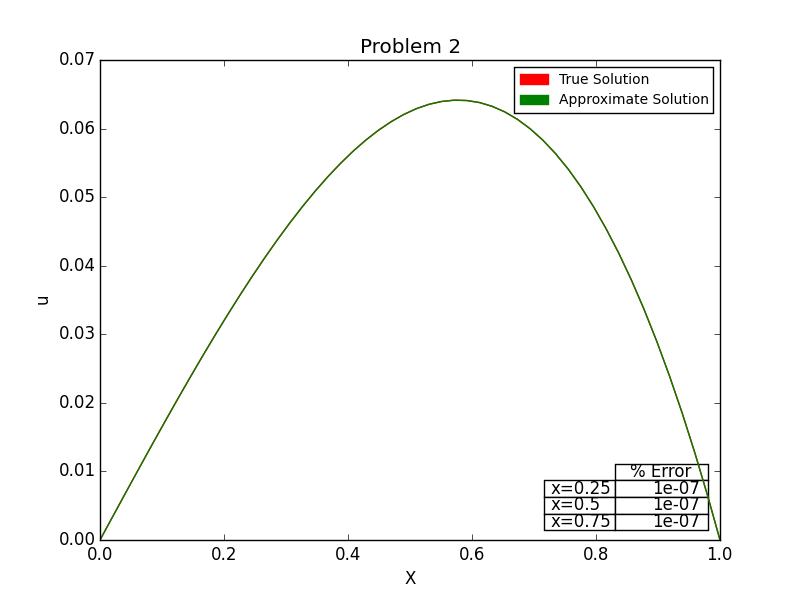
\includegraphics[scale=0.4]{two_poly_p2.png}
\end{center}

\tbf{C)} $\phi_1 \notin \mathcal{H}_0^1$ .
\section*{Problem 1 Part C Code.} What can Python do? It can do anything.

\begin{lstlisting}
from scipy import sin, cos, sinh
from scipy.integrate import quad as di
from numpy import pi, linspace, array
from numpy.linalg import solve as sls
import matplotlib.pyplot as plt
import matplotlib.patches as mpatches
import math

# Test Functions.
phi    = lambda x, c: sin(c*pi*x)
d_phi  = lambda x, c: c*pi*cos(c*pi*x)
phi2   = lambda x, c1, c2: phi(x, c1) * phi(x, c2)
d_phi2 = lambda x, c1, c2: d_phi(x, c1) * d_phi(x, c2)
f      = lambda x: x

# Parameters 
m = 0
M = 1
X    = linspace(m, M, 20)

# Real Solution
u = lambda x: x - sinh(x)/sinh(1)

# These functions generate matrix elements.
def K_(a, b, i, j):
    f = lambda x: phi2(x, i, j) + d_phi2(x, i, j)
    return di(f, a, b)[0]    

def F_(a, b, i):
    F = lambda x: f(x)*phi(x,i)
    return di(F, a, b)[0]

def plot_func(title, img_name, f, g, X, err):
    prec = 10000000
    plt.figure()
    plt.plot(X, f(X),'r' , X, g(X),'g')
    plt.title(title)
    plt.xlabel('X')
    plt.ylabel('u')
    red_patch = mpatches.Patch(color='red', label='True Solution')
    green_patch = mpatches.Patch(color='green', label='Approximate Solution')
    plt.legend(handles=[red_patch, green_patch], loc = 1, prop={'size':10})
    ax=plt.gca()
    col_labels=['% Error']
    row_labels=['x=0.25','x=0.5', 'x=0.75']
    table_vals=[[math.ceil(prec*err[0])/prec],[math.ceil(prec*err[1])/prec]\
        ,[math.ceil(prec*err[2])/prec]]
    # the rectangle is where I want to place the table
    the_table = plt.table(cellText=table_vals,
                      colWidths = [0.15],
                      rowLabels=row_labels,
                      colLabels=col_labels,
                      loc='lower right')
    plt.savefig(img_name)
    
# N = 1
alpha = F_(m, M, 1)/K_(m, M, 1, 1)
print alpha
u_approx = lambda x: alpha*phi(x,1)
err = [abs(u(0.25) - u_approx(0.25))/u(0.25), 
       abs(u(0.5) - u_approx(0.5))/u(0.5), 
       abs(u(0.75) - u_approx(0.75))/u(0.75)]
plot_func('One Basis Function', 'one.png', u, u_approx, X, err)

# N = 2
K = array([[K_(m, M, 1, 1), K_(m, M, 1, 2)],
            [K_(m, M, 2, 1), K_(m, M, 2, 2)]])
F = array([F_(m, M, 1),
            F_(m, M, 2)])
            
alpha = sls(K, F)
print alpha
u_approx = lambda x: alpha[0]*phi(x, 1) + alpha[1]*phi(x, 2)
err = [abs(u(0.25) - u_approx(0.25))/u(0.25),
       abs(u(0.5) - u_approx(0.5))/u(0.5),
       abs(u(0.75) - u_approx(0.75))/u(0.75)]
plot_func('Two Basis Functions', 'two.png', u, u_approx, X, err)

# N = 3
K = array([[K_(m, M, 1, 1), K_(m, M, 1, 2), K_(m, M, 1, 3)],
            [K_(m, M, 2, 1), K_(m, M, 2, 2), K_(m, M, 2, 3)],
            [K_(m, M, 3, 1), K_(m, M, 3, 2), K_(m, M, 3, 3)]])

F = array([F_(m, M, 1),
            F_(m, M, 2),
            F_(m, M, 3)])
            
alpha = sls(K, F)
u_approx = lambda x: alpha[0]*phi(x, 1) + alpha[1]*phi(x, 2) + alpha[2]*phi(x,3)
err = [abs(u(0.25) - u_approx(0.25))/u(0.25),
       abs(u(0.5) - u_approx(0.5))/u(0.5),
       abs(u(0.75) - u_approx(0.75))/u(0.75)]
plot_func('Three Basis Functions', 'three.png', u, u_approx, X, err)
\end{lstlisting}
\section*{Problem 1 Part D Codes.} This is essentially the same as the part c code, except I made some small changes to handle the polynomials.
\begin{lstlisting}
from scipy import sin, cos, sinh
from scipy.integrate import quad as di
from numpy import pi, linspace, array
from numpy.linalg import solve as sls
import matplotlib.pyplot as plt
import matplotlib.patches as mpatches
import math

# Test Functions.
p1  = lambda x: x*(1 - x)
p2  = lambda x: x*(1 - x)*(1.0/2.0 - x)
p3  = lambda x: x*(1 - x)*(1.0/3.0 - x)*(2.0/3.0 - x)
dp1 = lambda x: 1 - 2*x
dp2 = lambda x: 3*x**2 - 3*x + 1.0/2.0
dp3 = lambda x: 2.0/9.0 - 22.0*x/9.0 + 6*x**2 - 4*x**3

p11 = lambda x: p1(x)**2
p22 = lambda x: p2(x)**2
p33 = lambda x: p3(x)**2

p12 = lambda x: p1(x) * p2(x)
p13 = lambda x: p1(x) * p3(x)
p23 = lambda x: p2(x) * p3(x)

dp11 = lambda x: dp1(x)**2
dp22 = lambda x: dp2(x)**2
dp33 = lambda x: dp3(x)**2

dp12 = lambda x: dp1(x) * dp2(x)
dp13 = lambda x: dp1(x) * dp3(x)
dp23 = lambda x: dp2(x) * dp3(x)

f1 = lambda x: x*p1(x)
f2 = lambda x: x*p2(x)
f3 = lambda x: x*p3(x)

def dInt(fun):
    return di(fun, m, M)[0]
    
# Parameters 
m = 0
M = 1
X = linspace(m, M, 50)

# Real Solution
u = lambda x: x - sinh(x)/sinh(1)

def plot_func(title, img_name, f, g, X, err):
    prec = 10000000
    plt.figure()
    plt.plot(X, f(X),'r' , X, g(X),'g')
    plt.title(title)
    plt.xlabel('X')
    plt.ylabel('u')
    red_patch = mpatches.Patch(color='red', label='True Solution')
    green_patch = mpatches.Patch(color='green', label='Approximate Solution')
    plt.legend(handles=[red_patch, green_patch], loc = 1, prop={'size':10})
    ax=plt.gca()
    col_labels=['% Error']
    row_labels=['x=0.25','x=0.5', 'x=0.75']
    table_vals=[[math.ceil(prec*err[0])/prec],[math.ceil(prec*err[1])/prec],[math.ceil(prec*err[2])/prec]]
    # the rectangle is where I want to place the table
    the_table = plt.table(cellText=table_vals,
                      colWidths = [0.15],
                      rowLabels=row_labels,
                      colLabels=col_labels,
                      loc='lower right')
    plt.savefig(img_name)
    
# N = 1
i11 = lambda x: p11(x) + dp11(x)
alpha = dInt(f1)/dInt(i11)
u_approx = lambda x: alpha*p1(x)

err = [abs(u(0.25) - u_approx(0.25))/u(0.25), 
       abs(u(0.5) - u_approx(0.5))/u(0.5), 
       abs(u(0.75) - u_approx(0.75))/u(0.75)]
plot_func('1 Polynomial Basis Function', 'one_poly.png', u, u_approx, X, err)

# N = 2
i12 = lambda x: p12(x) + dp12(x)
i22 = lambda x: p22(x) + dp22(x)
K = array([[dInt(i11), dInt(i12)],
           [dInt(i12), dInt(i22)]])
F = array([dInt(f1),
           dInt(f2)])
            
alpha = sls(K, F)
u_approx = lambda x: alpha[0]*p1(x) + alpha[1]*p2(x)
err = [abs(u(0.25) - u_approx(0.25))/u(0.25),
       abs(u(0.5) - u_approx(0.5))/u(0.5),
       abs(u(0.75) - u_approx(0.75))/u(0.75)]
plot_func('2 Polynomial Basis Functions', 'two_poly.png', u, u_approx, X, err)


# N = 3
i13 = lambda x: p13(x) + dp13(x)
i23 = lambda x: p23(x) + dp23(x)
i33 = lambda x: p33(x) + dp33(x)
K = array([[dInt(i11), dInt(i12), dInt(i13)],
           [dInt(i12), dInt(i22), dInt(i23)],
           [dInt(i13), dInt(i23), dInt(i33)]])

F = array([dInt(f1),
           dInt(f2),
           dInt(f3)])
                       
alpha = sls(K, F)
u_approx = lambda x: alpha[0]*p1(x) + alpha[1]*p2(x) + alpha[2]*p3(x)
err = [abs(u(0.25) - u_approx(0.25))/u(0.25),
       abs(u(0.5) - u_approx(0.5))/u(0.5),
       abs(u(0.75) - u_approx(0.75))/u(0.75)]
plot_func('Three Polynomial Basis Functions', 'three_poly.png', u, u_approx, X, err)
\end{lstlisting}
\end{document}